\documentclass[a4paper,twoside,11pt,openright,table,draft]{article} %draft fuer nicht anzeigen der Bilder
\linespread{1.1} % Mehr abstand zwischen den Zeilen

%Diverses
\usepackage[table,xcdraw]{xcolor}  % for colored tables
\usepackage{layout} % just testing see later: \layout
\usepackage[top=2.7truecm,bottom=2.2truecm,inner=2.5cm,outer=3.5cm]{geometry}
\usepackage{lipsum} % just testing, filling pages with crap
\usepackage[english]{babel}
\usepackage[utf8]{inputenc}
\usepackage{amsmath}
\usepackage{enumitem}
\usepackage{graphicx}
\usepackage{wrapfig}
\usepackage[colorinlistoftodos]{todonotes}
\usepackage{epstopdf} % include eps
\usepackage{gensymb}
\usepackage{arydshln} % for dashed hlines
\newcommand{\rot}{\rotatebox[origin=l]{90}} % for rotation in table
\usepackage[nottoc]{tocbibind}
\usepackage{pdfpages} %pdf integrieren
\usepackage{hyperref} % For hyperlinks in the final pdf
\usepackage[T1]{fontenc} % fuer strange buchstaben
\usepackage[section]{placeins} % can use \FloatBarrier instead of clearpage
\setlength\parindent{0pt} % noindent fuer neue Paragraphen
\usepackage{multicol} % Für equations. side by side
\renewcommand{\labelitemi}{$-$} % Für itemize - verwenden


% For figures
\usepackage[skip=5pt]{caption} % changin length of caption with \captionsetup{width=.75\textwidth}
\usepackage{subcaption}
\renewcommand{\thefigure}{\arabic{figure}}
\renewcommand{\thesubfigure}{\Roman{subfigure}}
\captionsetup[figure]{labelformat = simple}
\captionsetup[subfigure]{labelformat=parens}

% Für grosses Layout drumherum
\usepackage{fancyhdr} 
% Für Header and Footings in Layout
\fancypagestyle{headings}{
	\fancyhf{}	
	\renewcommand{\headrulewidth}{0.4pt}
	\renewcommand{\footrulewidth}{0pt}
	\fancyhead[LO]{\nouppercase{\rightmark}} %leftmark
	\fancyhead[RE]{\nouppercase{Master's thesis}} % rightorleftmark Master's thesis leftmark see  http://mirrors.sorengard.com/ctan/macros/latex/contrib/fancyhdr/fancyhdr.pdf
	\fancyhead[LE,RO]{\thepage}
}
\setlength{\headheight}{14pt}
% if no subsection --> take section into the header
\makeatletter
\newcommand{\rightorleftmark}{%
  \begingroup\protected@edef\x{\leftmark}%
  \ifx\x\@empty
    \endgroup\rightmark
  \else
    \endgroup\leftmark
  \fi}
\makeatother

% Plain layout fuer Titelbild, ToC etc.
\fancypagestyle{plain}{
  \fancyhf{} % remove everything
  \renewcommand{\headrulewidth}{0pt} % remove lines as well
  \renewcommand{\footrulewidth}{0pt}
}
\makeatletter
\let\ps@plain\ps@empty
\makeatother

% Bibtex einbinden
\usepackage[
	backend=bibtex,
	style=authoryear,
	sorting=nyt,
	citestyle=authoryear-comp,
	maxcitenames=1,
	maxbibnames = 99,
	giveninits=true
	]{biblatex}
	
\addbibresource{Bib/Litverzeichnis.bib}
\setlength\bibitemsep{1.5\itemsep}
\DeclareNameAlias{sortname}{last-first}



\title{Photometric recording and modelling of the “Plan of St. Gall”} 
\author{Sabine Rüdisühli} 
\date{\today}

%% Start!!!
\begin{document}
\pagenumbering{roman} % Römische Zahlen für alles Vorgeplänkel (wird aber nicht im Layout dargestellt, nur für ToC)

\newgeometry{top=2.7truecm,bottom=2.2truecm,left=2.5truecm,right=2.5truecm}

\makeatletter
    \begin{titlepage}
    
\includegraphics[height = 10mm]{fig/ETH.png}% LogoETH.eps
    \hfill
    \quad
    
\includegraphics[height = 15mm]{fig/LogoIGP.png} \\[15ex]
        \begin{center}
            {\huge \bfseries  \@title }\\[9ex] 
            \begin{Large}
             {\textsc{Interdicipline Project Work }}\\[1ex]
              SS 2019 \\
			Zurich\\[5ex]       
                    \makeatother
                    \underline{Author} \\
                    Jon Allemand and Sabine Rüdisühli \\[2ex]
  					\makeatletter
  					\underline{Professorship} \\
  					Photogrammetry and Remote Sensing \\[2ex]
  					\underline{Supervision}\\
  					 Prof. Dr. Konrad Schindler \\[5ex]				
            \end{Large}
 		\end{center}     
    \end{titlepage}
\makeatother
\pagestyle{empty}
\cleardoublepage


\newgeometry{top=2.7truecm,bottom=2.2truecm,left=2.5truecm,right=3.5truecm}

\begin{abstract}
\noindent Abstract mit anderer Seiteneinrückung welche über "newgeometry" gelöst wird. Später wird die ursprüngliche geometrie mit ""restoregeometry" wieder zurückgeholt. \\
\end{abstract}

\renewcommand{\abstractname}{Acknowledgements}
\begin{abstract}
\noindent We would like to sincerely thank Professor Schindler, because he made possible an extraordinary project that brought together our acquired technical knowledge and a cultural asset. In addition, for the simple, but still very good care. Furthermore, we sincerely thank the whole Stiftsbibliothek of St. Gall, who received us a very warm welcome and a great confidence to work with the unique plan. Very big help was the Abbey librarian Cornel x, who made all the impossible things possible, and Silvio y, who was always available for our questions and made the whole measuring process possible.\\
\end{abstract}
\cleardoublepage

\restoregeometry

\tableofcontents
\clearpage

\listoffigures
\listoftables
\cleardoublepage

\pagestyle{headings}
\renewcommand{\subsectionmark}[1]{\markright{\thesubsection\ #1}}

\layout % for showing how the layout is now defined

\section{Introduction}
\pagenumbering{arabic}
\setcounter{page}{1}
The start of the painting of the Plan of Saint Gall was in 16xx and afterwards, new parts were added. Due to the lifetime and the painting the plan gets some “injuries”. To detect traces of the past, the Plan was recorded with the best measurement system nowadays, the Minidome, which allows to measure with mm-submilitre resolution and in 2.5D. 

To substract some information from the Plan, firstly, the patches recording have to be stitched together. This steps have to be done because the portable Minidome can only record patches of a size of x X x cm and the Plan has a totally size of  x m. For the extracting of research features, ideas have to build up which should work on an old, crumbled plan. These detected features will be afterwards analysed from plan experts. 
To prepare information for the experts, the plan was stitched together with Photoshop because all other program reached their limits with the given 1.5 TB dataset. The key point in this step was to get the transform parameters for each patch. After a lot of tries, Finally, a self-written C++ script solved the program. The second challenge, extracting research features like needle holes and scratches, can be only solved with manual detecting because the crumbled old plan destroyed all the genius, theoretical ideas for detecting. For examples, the made assumption that needle holes should be round and have some height differences are logical, but the circle matching program gave a lots of more possible circles which lays in wrinkled regions.
 \\
"textcite{}" für in den Fliesstext ergibt "\textcite{Dobbertin2005}" \newline
"parencite{}" für in der Klammer ergibt "\parencite{Dobbertin2005}"


Neue Linie mit doppelbackslash oder "newline" Befehl oder zwei Absätzen. \newline


"quote": Wie man etwas wörtlich zitieren kann so dass es schön formatiert ist:
\begin{quote}However blabla bla on average small.
\end{quote}


Ein externes Latex-Dokument einbinden ist ganz einfach mit "input" zu bewältigen:

%notmain.tex

Dies ist in einem separaten .tex Dokument namens notmian.tex abgespeichert.\\

 
Eine Aufzählung machen...
\begin{itemize}
	\item item one
	\item item two
\end{itemize}

und mit weniger Abstand:
\begin{itemize}[noitemsep]
	\item item one
	\item item two
\end{itemize}


Italics mit "textit" \textit{dies ist schraeggestellt}\\

Url einfügen und Footnote mit Accessdatum \url{https://deephunt.in/the-gan-zoo-79597dc8c347}\footnote{accessed: 05.06.2018}.\\
Schwarzer Balken am Ende der Zeile wird angezeigt da wir im Draft-Modus sind, zeigt an, dass wir eine unschöne überlänge haben...


"ref" für automatische Verweise welche mit "label" beim Objekt definiert werden. Benamsung mit prefixen wie: "sec:" (section), "fig:" (figure) tab: (Tabelle) helfen übersicht zu behalten.\\
Beispiel: siehe für weiteres in Section \ref{sec:second_section}.\\

"cleardoublepage" wenn "twosides" (d.h. wenn doppelseitig bedruckt werden soll) damit der neue Abschnitt wieder auf der Rechtenseite neu anfängt.\\
"clearpage" wenn neue Seite angefangen werden soll\\
"FloatBarrier" aus package "placeins" macht, dass einfach alle noch herumliegenden Bilder eingefügt werden...\\
"newpage" macht irgendwie auch eine neue Seite...\\


Beispiel Tabelle und Figuren mit package subcaption
\begin{table}[!hbt]
	\centering
	\caption{\label{tab:Ur_human_img}Quantification of errors for the images in Figure \ref{fig:Ur_human_img}.}
	\begin{tabular}{|l|c|c|c|c|c|r|}
	\hline
	Name                  & I    & II   & III  & IV   &  V   & VI   \\ \hline
	Standard deviation    & 15.8 & 16.3 & 17.4 & 16.0 & 15.7 & 16.5 \\ \hline
	Smallest defoliation  & 25   & 30   & 35   & 10   & 15   & 20   \\ \hline
	Highest defoliation   & 70   & 75   & 80   & 50   & 60   & 65   \\ \hline
	\end{tabular}
\end{table}

\begin{figure}[!htb]
	\centering
	\begin{subfigure}{0.32\textwidth}
		\centering
		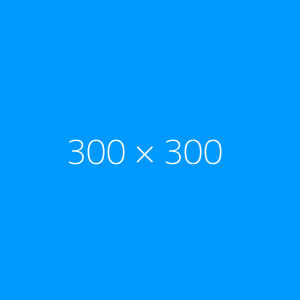
\includegraphics[width=0.85\textwidth]{fig/dummy.png}
		\caption{}
	\end{subfigure}
	\begin{subfigure}{0.32\textwidth}
		\centering
		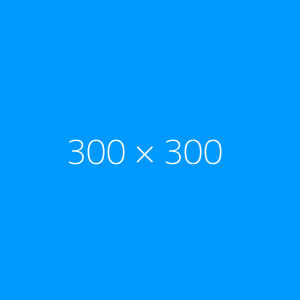
\includegraphics[width=0.85\textwidth]{fig/dummy.png}
		\caption{}
	\end{subfigure}
	\begin{subfigure}{0.32\textwidth}
		\centering
		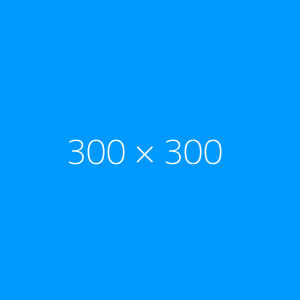
\includegraphics[width=0.85\textwidth]{fig/dummy.png}
		\caption{}
	\end{subfigure}
	\begin{subfigure}{0.32\textwidth}
		\centering
		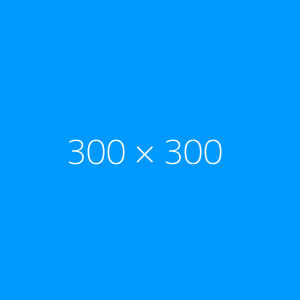
\includegraphics[width=0.85\textwidth]{fig/dummy.png}
		\caption{Mit Text}
	\end{subfigure}
	\caption[Difficult trees to estimate defoliation for]{\label{fig:Ur_human_img}Trees that caused the highest deviations in the estimations.}
\end{figure}


\begin{figure}[!htb]
	\centering
	\begin{subfigure}{0.49\textwidth}
	\captionsetup{width=.9\linewidth}
		\centering
		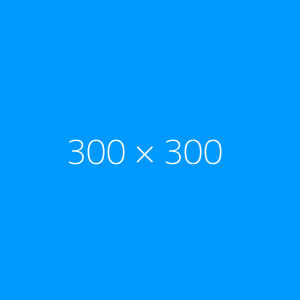
\includegraphics[width=0.95\textwidth]{fig/dummy.png}
		\caption{Error curves showing the accuracy of the different observers.}
	\end{subfigure}
	\begin{subfigure}{0.49\textwidth}
		\captionsetup{width=.9\linewidth}
		\centering
		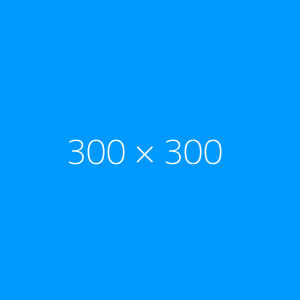
\includegraphics[width=0.95\textwidth]{fig/dummy.png}
		\caption{Distribution of predicted values to ground-truth for my personal estimation.}
	\end{subfigure}
	\caption[Human estimation of defoliation]{\label{fig:Ur_human_cum}}
\end{figure}

\newpage

Zwei Kolonnen nebeneinander mit Formeln:
\begin{multicols}{2}
\begin{equation} \label{eq:l2loss}
	L_{i} = || f - y_{i} ||^{2}_{2} = \sum\limits_{j} ( f_{j} -(y_{i})_{j})^{2}
\end{equation} \break
\begin{equation} \label{eq:l1loss}
	L_{i} = || f - y_{i} ||_{1} = \sum\limits_{j} | f_{j}-(y_{i})_{j}|
\end{equation}
\end{multicols}

\FloatBarrier

Zum Text um Figure umfliessen lassen:\\
\begin{wrapfigure}{R}{0.5\textwidth}
	\centering
	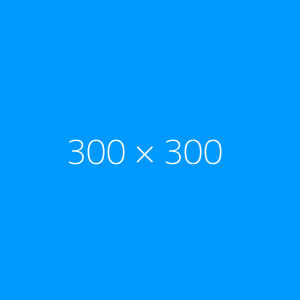
\includegraphics[width=0.45\textwidth]{fig/dummy.png}
	\caption[Basic structure of a CNN]{\label{fig:overview_cnn}Basic structure of a CNN.(Adabted from: \textcite{chollet2017})}
\end{wrapfigure}

\lipsum[1-2]
\cleardoublepage

\section{Measurement}
\label{sec:second_section}
\lipsum[2]
\subsection{Setup}
\lipsum[2]
\subsection{Minidome}
\lipsum[7]
\subsubsection{Shape of Shading}
\lipsum[8]
\subsubsection{Data}
\lipsum[9]
\cleardoublepage

\clearpage
\section{Stitiching}
\label{sec:third_section}

\clearpage
\section{Feature detection}
\label{sec:four_section}

\subsection{Needle holes}
\subsubsection{Scientific Approach}
\subsubsection{Reality}


\subsection{Scratches}


\clearpage
\section{Conclusion}
Blabla

\printbibliography[heading=bibintoc] %\todo
\cleardoublepage

\appendix
\section{Appendix}
Appendix blabla

\pagestyle{empty}
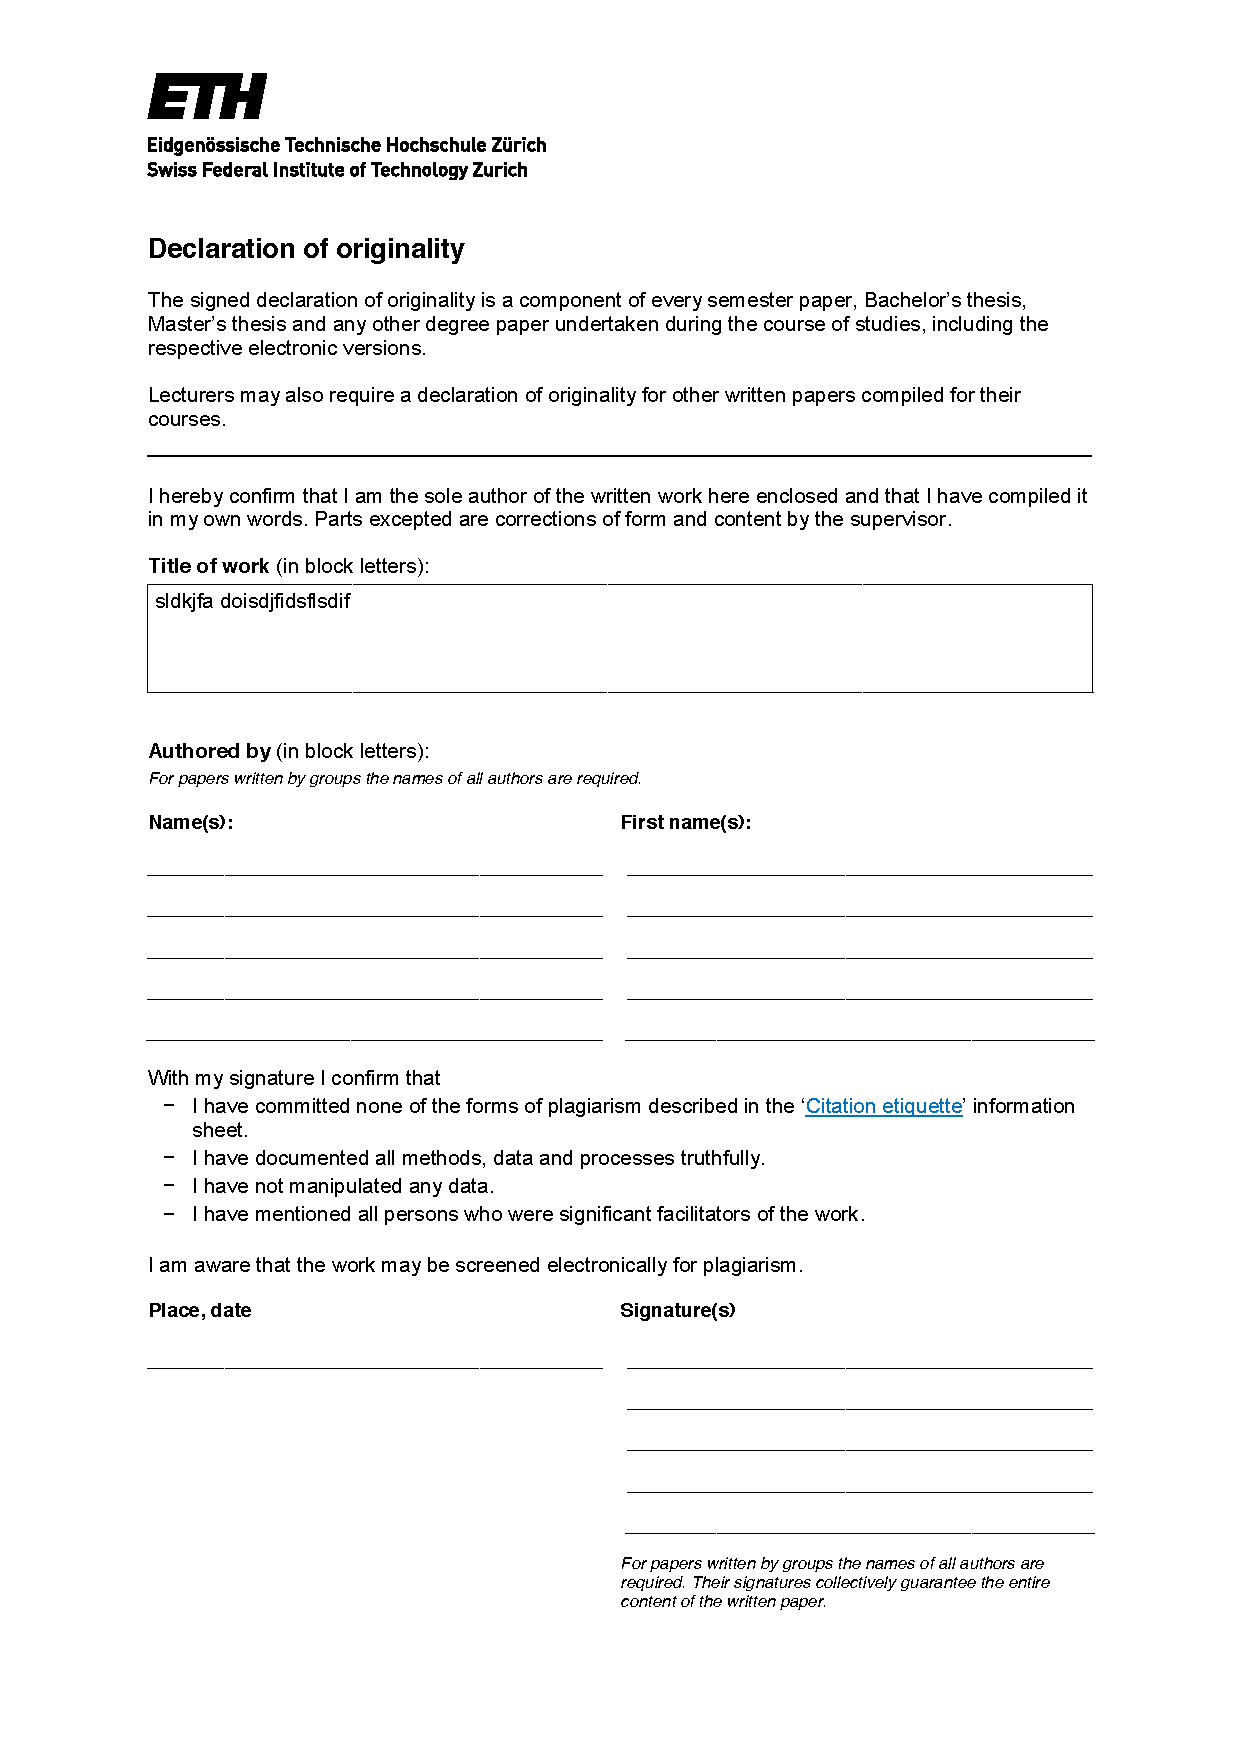
\includepdf[pagecommand = {}]{pdf/dec_dummy.pdf}

\end{document}
